\documentclass{report}
\usepackage[left=4.5cm, right=2cm, top=3cm]{geometry}
\usepackage[latin1]{inputenc}
\usepackage[spanish]{babel}
\usepackage{graphicx}
\usepackage{amssymb}
\usepackage{dsfont}
\usepackage{amsmath}
\usepackage{amsthm}
\usepackage{fancyhdr}
\usepackage{xpatch}
\usepackage{xcolor}
\usepackage{centernot}
\usepackage{hyperref}
\usepackage{mathtools}
\usepackage[many]{tcolorbox} %Hacer las cajitas de observaciones
\usepackage{setspace} %Cambiar interlinados del titulo
\usepackage{bbm} %Para poner la indicadora
\usepackage{mathtools} %para la flechita con letras

%%%%%%%%%%%%%%%%%%%%%%%COMANDOS USUALES QUE USAS%%%%%%%%%%%%%%%%%%%%%%%%%%%%%
\xpatchcmd{\proof}{\itshape}{\normalfont\proofnamefont}{}{}
\newcommand{\proofnamefont}{\bfseries} %Ambiente 'Prueba' (Proof) sale la palabra 'Proof' (Demostraci�n) en negritas. [Creo]
\newcommand{\indep}{\rotatebox[origin=c]{90}{$\models$}} %Simbolo de independientes
\linespread{1.2} %Iterlineado
\DeclarePairedDelimiter\ceil{\lceil}{\rceil}
\DeclarePairedDelimiter\floor{\lfloor}{\rfloor}
\renewcommand{\baselinestretch}{1.5}  %Este sirve para inetrlineados del titulo
\newenvironment{boldenv} %poner en negritas la pregunta
  {\bfseries}% \begin{boldenv}
  {}% \end{boldenv}
\newenvironment{respuesta}{\paragraph{Respuesta}}{\hfill$\triangle$\\} %ambiente 'respuesta'
%%%%%%%%%%%%%%%%%%%%%%%%%%%%%%%%%%%%%%%%%%%%%%%%%%%%%%%%%%%%%%%%%%%%%%%%%%%%%%

%-----------------------titulo
\title{Maestr�a en Ciencia de Datos.\\ Matem�ticas para Ciencia de Datos.}
\author{Mar�a Elena Mart�nez Manzanares}
\date{Septiembre 2022}
%-----------------------------



\begin{document}

	\pagestyle{fancy}
	\fancyhf{}
	\rhead{\thepage}
	\maketitle

	{\Large\textbf{Parte 1}}
	
\begin{boldenv}
	Considera la matriz
	\begin{equation*}
	M:=
		\begin{pmatrix}
		1&1&2&1\\
		0&0&0&1\\
		1&2&2&1\\
		\end{pmatrix}
\end{equation*}
Sea $A$ la matriz formada con las dos primeras columnas de $M$. Describe:
\begin{description}
	\item[1.] el dominio y el codominio de $A$ como transformaci�n lineal.
	\item[2.] la imagen de $A$ y el kernel de $A$.
	\item[3.] la imagen de $A^T$ y el kernel de $A^T$.
\end{description}
\end{boldenv}
	\noindent\textbf{Respuesta.}
	
	\textbf{(1)} El dominio es $\mathbb{R}^2$ y el codominio es $\mathbb{R}^3$.
	
	\textbf{(2)} Dado que $(1,0,1)^T$ y $(1,0,2)^T$ son linealmente independientes, tenemos que la imagen es
	\begin{equation*}
		\textrm{span}\left\{(1,0,1)^T,(1,0,2)^T\right\}.
	\end{equation*}
	Por el Teorema del Rango y la Nulidad tenemos que
	\begin{equation*}
		\textrm{Rango}(A) + \textrm{Nulidad}(A)=2,
	\end{equation*}
	esto implica que Nulidad$(A)=0$, por lo que el Kernel consiste solamente del vector cero.
	
	\textbf{(3)} Notemos que $A^T =
		\begin{pmatrix}
			1&0&1\\
			1&0&2\\
		\end{pmatrix}$. Esto implica que
	\begin{equation*}
		\textrm{Im}(A)=\textrm{span}\left\{(1,1)^T,(1,2)^T\right\}.
	\end{equation*} 
	De nueva cuenta por el Teorema del Rango y la Nulidad, se deduce que Nulidad$(A^T)=1$. Analizamos la matriz $A^T$ para buscar el vector que genera el kernel.
	\begin{equation}\label{ec1}
		\begin{pmatrix}
			1&0&1\\
			1&0&2\\
		\end{pmatrix}
		\begin{pmatrix}
			x_1\\
			x_2\\
			x_3\\
		\end{pmatrix}=
		\begin{pmatrix}
			0\\
			0\\
		\end{pmatrix}.
	\end{equation}
	Por medio de matrices elementales podemos llegar a que (\ref{ec1}) es equivalente al sistema
		\begin{equation*}
		\begin{pmatrix}
			1&0&0\\
			0&0&1\\
		\end{pmatrix}
		\begin{pmatrix}
			x_1\\
			x_2\\
			x_3\\
		\end{pmatrix}=
		\begin{pmatrix}
			0\\
			0\\
		\end{pmatrix}.
	\end{equation*}
	Esto implica que $x_1=x_3=0$. Esto implica que 
	\begin{equation*}
		\textrm{Kernel}(A)=\textrm{span}\left\{(0,1,0)^T\right\}.
	\end{equation*}
	
	\vspace{0.5cm}
	\begin{boldenv}
	Decide si la transformaci�n $A$ es sobre, uno-a-uno, o ninguna de las dos anteriores. Adem�s, note que claramente la tercera columna de $M$ es una combinaci�n lineal de las dos anteriores
	\begin{equation*}
	\textrm{col}_{3}=2\textrm{col}_1+0\textrm{col}_2.
	\end{equation*}
	Encuentra esa respuesta por medio de la pseudoinversa de $A$.
	\end{boldenv}
	
		\noindent\textbf{Respuesta.}
		Notemos que $A:\mathbb{R}^2\rightarrow \mathbb{R}^3$. Por lo demostrado anteriormente, sabemos que $\textrm{Nulidad}(A)=0$, por lo tanto es 1-1. La matriz no es sobreyectiva ya que $\textrm{Rango}(A)=2$
		
		Por otro lado, nos interesa determinar el vector $\alpha=(\alpha_1,\alpha_2)^T$ tal que
		\begin{equation*}
			A
		\begin{pmatrix}
			\alpha_1\\
			\alpha_2\\
		\end{pmatrix}
		=
		\textrm{col}_3.
		\end{equation*}
		La pseudoinversa por la izquierda de $A$, $A^{+}=(A^TA)^{-1}A^T$ es
		\begin{equation*}
		\begin{pmatrix}
			2 & 0 & -1 \\
			-1 & 0 & 1
		\end{pmatrix}.
		\end{equation*}
			Esto implica que 
			\begin{eqnarray*}
				\alpha&=&A^{+}\textrm{col}_3,\\
							&=&
		\begin{pmatrix}
			2 & 0 & -1 \\
			-1 & 0 & 1
		\end{pmatrix}
		\begin{pmatrix}
		2\\
		0\\
		2\\
		\end{pmatrix},\\
		&=&\left(2,0\right)^T.
			\end{eqnarray*}
			Es decir,
			\begin{equation*}
			2\textrm{col}_1+0\textrm{col}_2=\textrm{col}_3.
			\end{equation*}
		
		\vspace{0.5cm}
		\begin{boldenv}
			Sea ahora $A$ la matriz formada con los dos primeros renglones de $M$. Describe:
				\begin{description}
					\item[1.] el dominio y el codominio de $A$ como transformaci�n lineal.
					\item[2.] la imagen de $A$ y el kernel de $A$.
					\item[3.] la imagen de $A^T$ y el kernel de $A^T$.
				\end{description}			 
		\end{boldenv}
		\noindent\textbf{Respuesta.}
	
	\textbf{(1)} El dominio es $\mathbb{R}^4$ y el codominio es $\mathbb{R}^2$.
	
	\textbf{(2)} La matriz $A$ esta formada por dos columnas linealmente independientes, por lo que la imagen es todo $\mathbb{R}^2$. Analizamos la matriz para determinar el kernel
	\begin{equation*}
	\begin{pmatrix}
		1&1&2&1\\
		0&0&0&1\\
	\end{pmatrix}
	\begin{pmatrix}
		x_1\\
		x_2\\
		x_3\\
		x_4\\
	\end{pmatrix}
	=
	\begin{pmatrix}
		0\\
		0\\
	\end{pmatrix}.
	\end{equation*}
	De este planteamiento se sigue inmediatamente que $x_4=0$. Por otro lado, obtenemos que $x_1=-x_2-2x_3$. Esto implica que la soluci�n viene dada por $(-x_2-2x_3,x_2,x_3,0)^T$. Por lo tanto, el kernel es
	\begin{equation*}
		\textrm{span}\left\{(-1,1,0,0)^T,(-2,0,1,0)^T\right\}.
	\end{equation*}
	
	\textbf{(3)} Notemos que $A^T$ es la matriz
	\begin{equation*}
	\begin{pmatrix}
	1&0\\
	1&0\\
	2&0\\
	1&1
	\end{pmatrix}.
	\end{equation*}
	Esta matriz tiene dos columnas linealmente independientes, por lo que su imagen es
	\begin{equation*}
		\textrm{span}\left\{(-1,1,0,0)^T,(-2,0,1,0)^T\right\}.
	\end{equation*}
	
	El kernel consiste solamente del vector cero debido a que del Teorema del Rango y la Nulidad se sigue que
	\begin{equation*}
		2=\textrm{Rango}(A^T)+\textrm{Nulidad}(A^T)=2+\textrm{Nulidad}(A^T).
	\end{equation*}
	y esto implica que la dimensi�n del kernel de la matriz $A^T$ es cero.
	\vspace{0.5cm}
	
	
	\begin{boldenv}
		Decide si la transformaci�n es sobre, uno-a-uno, o ninguna de las dos anteriores. Describe al conjunto de soluciones $Ax=b$ donde $b=(6,0)^T$. �Puedes encontrar una soluci�n espec�fica $x^{+}$ por medio de la pseudoinversa? Hint: Las soluciones de $Ax=b$ es el conjunto:
		\begin{equation*}
			x_{\textrm{esp}}+\textrm{Ker}A = \{x=x_{\textrm{esp}}+x_{\textrm{null}}: x_{\textrm{null}}\in\textrm{Ker}(A)\}
		\end{equation*}
		donde $x_{\textrm{esp}}$ es una soluci�n espec�fica de $Ax=b$. �Este conjunto es independiente de la soluci�n expec�fica que se use para la descripci�n!
	\end{boldenv}
	\noindent\textbf{Respuesta.}
	
	La matriz no es uno-a-uno porque su kernel es distinto del vector cero. Por otro lado, la matriz si es sobreyectiva porque su imagen es $\mathbb{R}^2$. 
	
	Notemos que
	\begin{eqnarray*}
		Ax&=&b,\\
			\begin{pmatrix}
		1&1&2&1\\
		0&0&0&1\\
	\end{pmatrix}
	\begin{pmatrix}
		x_1\\
		x_2\\
		x_3\\
		x_4\\
	\end{pmatrix}
	&=&
	\begin{pmatrix}
		6\\
		0\\
	\end{pmatrix}.
	\end{eqnarray*}
	Esto implica que $x_4=0$. Por lo tanto, $x_1=6-x_2-2x_3$. La soluci�n general es $(6-x_2-2x_3,x_2,x_3,0)$. Para encontrar una soluci�n espec�fica por medio de la pseudoinversa, considerando que $A$ es sobreyectiva tenemos que la pseudoinversa por la derecha es $A^{+}=A^T(AA^T)^{-1}$, por lo tanto
	\begin{eqnarray*}
	x&=&A^{+}b,\\
		&=&\begin{pmatrix}
			\frac{1}{6} & \frac{-1}{6} \\
			\frac{1}{6} & \frac{-1}{6} \\
			\frac{1}{3} & \frac{-1}{3} \\
			0 & 1
		\end{pmatrix}
		\begin{pmatrix}
			6\\
			0\\
		\end{pmatrix}\\
		&=&
		\begin{pmatrix}
			1\\
			1\\
			2\\
			0
		\end{pmatrix}.
	\end{eqnarray*}
	Esto significa que
	\begin{equation*}
		\textrm{col}_1+\textrm{col}_2+2\textrm{col}_3 = (6,0)^T
	\end{equation*}
	y $x^{+}=(1,1,2,0)^{T}$ es una soluci�n espec�fica.
	
	\newpage
	{\Large \textbf{Parte 2}}
	
	\begin{boldenv}
		Demuestra que $A$ es uno-a-uno si y s�lo si $A^T$ es sobre.
	\end{boldenv}
	\begin{proof}
		\noindent $(\Rightarrow)$. Supongamos que $A:\mathbb{R}^n\rightarrow\mathbb{R}^m$ es uno-a-uno. Eso significa que Kernel$(A)=0$, lo cual implica por el Teorema del Rango y la Nulidad que Rango$(A)=n$. Por el resultado final de la lista de ejercicios, tenemos que $n=$Rango$(A)=$Rango$(A^T)$, y $A^T:\mathbb{R}^m\rightarrow \mathbb{R}^n$, esto significa que Rango$(A^T)=\textrm{Rango}(\mathbb{R}^n)$ y por lo tanto $A^T$ es sobre.
		
		\noindent $(\Leftarrow)$. Supongamos que $A^T:\mathbb{R}^m\rightarrow\mathbb{R}^n$ es sobreyectiva. Esto implica que $\textrm{Rango}(A^T)=n$. Por el resultado final de la lista de ejercicios, tenemos que $\textrm{Rango}(A^T)=\textrm{Rango}(A)$. Por el Teorema del Rango y la Nulidad tenemos que 
		$n=\textrm{Nulidad}(A)+\textrm{Rango}(A)=\textrm{Nulidad}(A)+n$, de lo cual se sigue que $\textrm{Nulidad}(A)=0$ y por lo tanto $A$ es 1-1.
	\end{proof}
	
		\begin{boldenv}
		Prueba en una l�nea que Ran $A$ es ortogonal a Ker $A^T$ en el sentido de que cada vector en Ran $A$ es ortogonal a cada elemento del Ker $A^T$.
	\end{boldenv}
	\begin{proof}
		Sea $v\in \textrm{Ran}(A)$. Entonces existe $z\in \textrm{Dom}(A)$ tal que $Az=v$. Sea $w\in\textrm{Ker}(A^T)$.  Notemos que
		\begin{equation*}
			<v,w>=<Az,v>=<z,A^Tv>=<z,0>=0.
		\end{equation*}
	\end{proof}
	
	\begin{boldenv}
		Prueba que si las columnas de una matriz $A$ forman un conjunto linealmente independiente entonces $A^TA$ es invertible.
	\end{boldenv}
	\begin{proof}
		Supongamos que $A:\mathbb{R}^n\rightarrow\mathbb{R}^m$ tiene columnas linealmente independientes. La matriz $A^TA:\mathbb{R}^n\rightarrow \mathbb{R}^n$, por lo que es un operador de $\mathbb{R}^n$. Para demostrar que es invertible, basta entonces demostrar que es 1-1. Supongamos que $x\in\mathbb{R}^n$ es tal que $A^TAx=0$. Por lo demostrado en un ejercicio m�s adelante, tenemos que $A$ y $A^TA$ tienen el mismo espacio nulo, eso implica que $Ax=0$. Como $A$ tiene columnas linealmente independientes, $Ax=0$ implica que $x=0$.
	\end{proof}
	
	\begin{boldenv}
		Sea $w$ un vector en $\mathbb{R}^n$ para alg�n $n$ y $b\in\mathbb{R}$. Considere el conjunto de todos $x$ tales que
		\begin{equation*}
			<w,x>=b.
		\end{equation*}
		Da una descripci�n geom�trica de este conjunto en t�rminos de $w$ y $b$.
	\end{boldenv}
	\begin{respuesta}
		Podemos considerar la transformaci�n $f(x)=<w,x>$, $f:\mathbb{R}^n\rightarrow\mathbb{R}$, la cual es lineal debido a la linealidad del producto interior. Si tenemos un escalar $b$ de tal manera que $f(x)=b$, entonces en este caso particular $f$ tendr� la representaci�n de un hiperplano que en el origen toma el valor $b$ y que divide el espacio en dos (por arriba del hiperplano, $f(x)>0$, y por debajo de el, $f(x)<0$).
	\begin{center}
	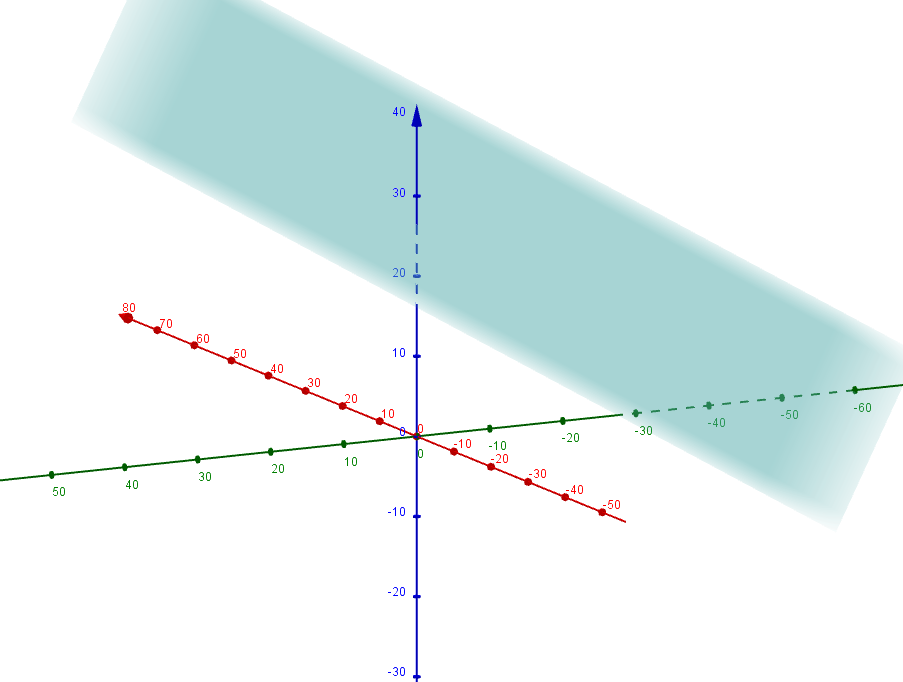
\includegraphics[height=5cm]{plano_afin.PNG}
	\end{center}
	
	Cuando $b=0$, el plano en el origen toma el valor $0$ y en este caso el hiperplano es un subespacio vectorial que divide el espacio en dos.
	\begin{center}
	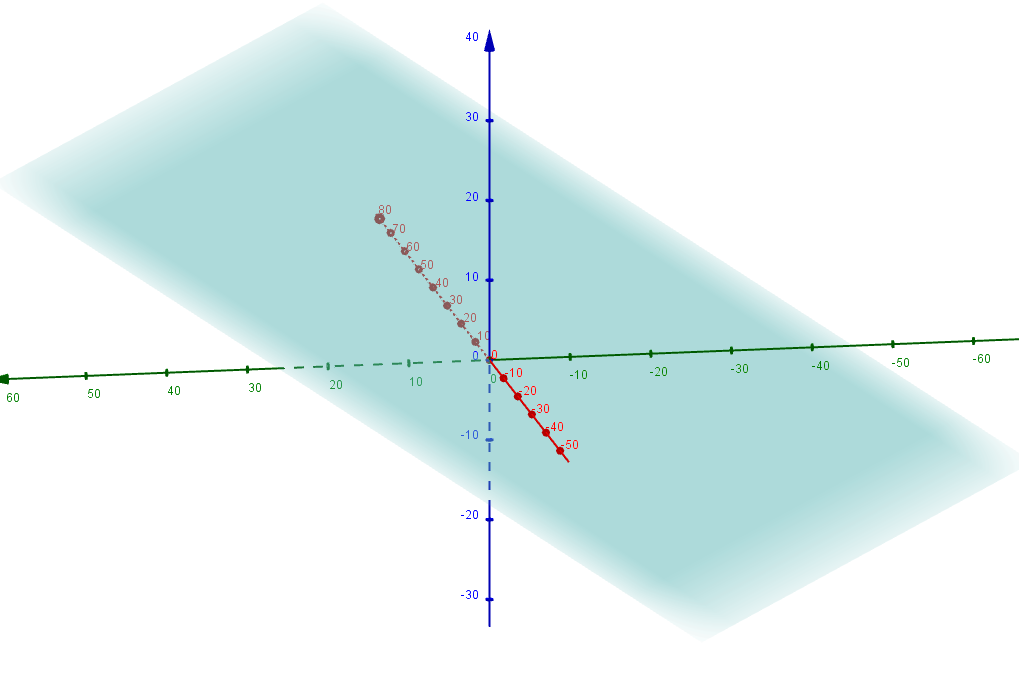
\includegraphics[height=5cm]{espacio_vec.PNG}
	\end{center}	
	\end{respuesta}
	
	\begin{boldenv}
		Verifica que $\textrm{Rango}A=\textrm{Rango}A^T=\textrm{Rango}(A^TA)=\textrm{Rango}(AA^T)$.
	\end{boldenv}
	\begin{proof}
	Sea $x\in \textrm{Dom}(A)$.
	
	Demostraremos que $\textrm{Rango}A=\textrm{Rango}(A^TA)$, si demostramos que $\textrm{Kernel}A=\textrm{Kernel}(A^TA)$ y consideramos el Teorema del Rango y la Nulidad. Notemos que
	\begin{eqnarray*}
		A^TAx&=&0,\textrm{ multiplicando por $x^T$ a ambos lados}\\
		x^TA^TAx&=&0,\\
		(Ax)^TAx&=&0,\\
		<Ax,Ax>&=&0,\\
		||Ax||^2&=&0.
	\end{eqnarray*}
	Esto implica que $Ax=0$ y por lo tanto $\textrm{Kernel}(A^TA)\subset \textrm{Kernel}A$. La otra contenci�n es trivial. 
	
	Sea $y\in \textrm{Dom}(A^T)$. De manera an�loga demostraremos ahora que $\textrm{Rango}A^T=\textrm{Rango}(AA^T)$
	\begin{eqnarray*}
		AA^Ty&=&0,\textrm{ multiplicando por $y^T$ a ambos lados}\\
		y^TAA^Ty&=&0,\\
		(A^Ty)A^Ty&=&0\\
		<A^Ty,A^Ty>&=&0,\\
		||A^Ty||^2&=&0.
	\end{eqnarray*}
	Esto implica que $A^Ty=0$ y por lo tanto $\textrm{Kernel}(AA^T)\subset \textrm{Kernel}A^T$. La otra contenci�n es trivial. 
	
	Finalmente, demostraremos que $\textrm{Rango}A=\textrm{Rango}A^T$. Por lo que demostramos antes, tenemos
	\begin{equation*}
		\textrm{Rango}(A)=\textrm{Rango}(A^TA)\leq \textrm{Rango}(A^T)
	\end{equation*}
	donde la �ltima desigualdad es debido a que $A^TA$ es una combinaci�n lineal de las columnas de $A^T$. Similarmente, tenemos que
	\begin{equation*}
		\textrm{Rango}(A^T)=\textrm{Rango}(AA^T)\leq \textrm{Rango}(A).
	\end{equation*}
	Por lo tanto, $\textrm{Rango}A=\textrm{Rango}A^T$.
	\end{proof}
\end{document}